\section{Introduction}
On présente dans ce document le calcul du groupe fondamental de $3$ surfaces : le tore $T^2$, le plan projectif réel $\mathbb{R}$P$^2$ et la bouteille de Klein $K$.\\
\begin{figure}[h]
    \begin{minipage}{0.32\textwidth}
        \centering
        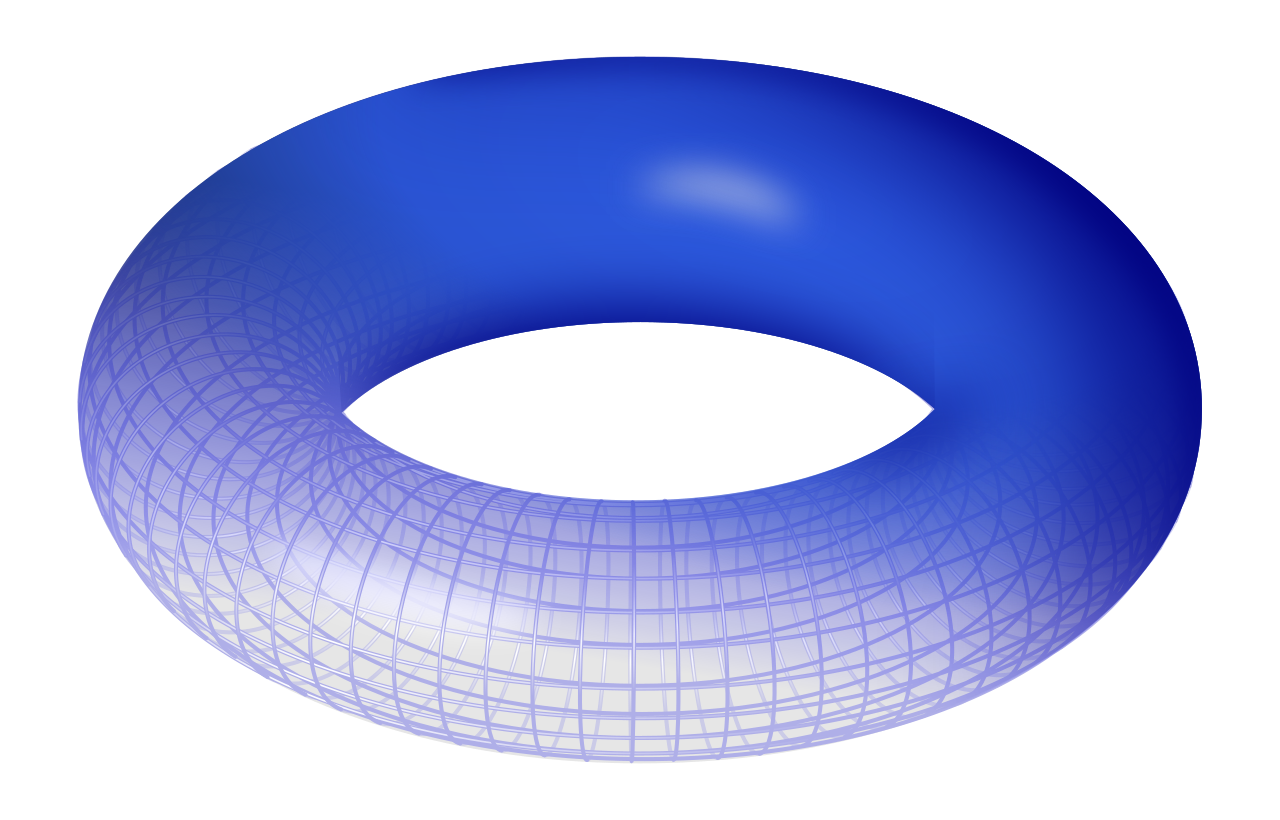
\includegraphics[width=\linewidth]{images/tore exemple.png}
    \end{minipage}
    \hfill
    \begin{minipage}{0.32\textwidth}
        \centering
        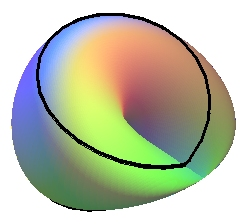
\includegraphics[width=\linewidth]{images/rp2 exemple.jpg}
    \end{minipage}
    \hfill
    \begin{minipage}{0.32\textwidth}
        \centering
        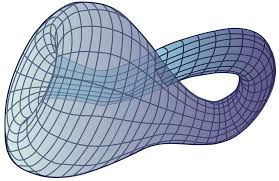
\includegraphics[width=\linewidth]{images/klein exemple.jpg}
    \end{minipage}
    \caption{Le tore, le plan projectif et la bouteille de Klein, dans l'ordre.}
\end{figure}
\medskip\\
Le groupe fondamental $\pi_1$ est formé à partir des classes d'homotopies des lacets de ces surfaces. En identifiant ces dites surfaces à des carrés dont on recolle les bords, on va appliquer le théorème de Van Kampen pour obtenir des isomorphismes à des groupes que l'on sait étudier.\medskip\\
Ainsi, pour le tore par exemple on va déterminer que son groupe fondamental $\pi_1(T^2)$ est isomorphe à $\mathbb{Z}\times\mathbb{Z}$, ce qui se comprend intuitivement en caractérisant un lacet déterminé à homotopie près par un nombre de tours passant par le trou au centre, et un deuxième nombre de tours longeant le tore.\medskip\\
Ce qui est pratique avec ces $3$ surfaces, c'est que la méthode utilisée pour calculer leur groupe fondamental est plutôt similaire. On va donc d'abord établir des résultats un peu plus généraux, qui s'appliqueront à ces surfaces, pour ensuite procéder au calcul de manière plus confortable.\medskip\\
Ce texte ne faisant pas office d'introduction à la topologie algébrique ou à l'étude des homotopies, on suppose quelques résultats déjà connus. Ils sont tous retrouvables dans le livre Algebraic Topology de Hatcher, que j'ai étudié pour m'introduire au sujet. On va commencer par les énumérer, puis on démontrera quelques résultats utiles. Ensuite, on calculera dans l'ordre les groupes fondamentaux de $T^2$, puis de $\mathbb{R}$P$^2$ et on finira par $K$. Après cela, on récapitulera les propriétés obtenues, et on proposera d'exécuter le code python présent dans le projet, mettant en œuvre une visualisation des surfaces ainsi étudiées.
\subsection{Résultats préliminaires}
On admettra dans ce document des résultats théoriques de base. On les énumère ici :\medskip\\
- Si $X$ et $Y$ sont des espaces topologiques homéomorphes, alors ils vérifient $\pi_1(X)\cong\pi_1(Y)$.\medskip\\
- Si $A\subset X$ est un retract par déformation de $X$, alors $\pi_1(A)\cong\pi_1(X)$.\medskip\\
- Le groupe fondamental du cercle est isomorphe à $(\mathbb{Z},+)$. Autrement dit, $\pi_1(S^1)\cong\mathbb{Z}$.\medskip\\
On rappelle aussi l'énoncé du théorème de Van Kampen, avec la précision que $i_{\alpha\beta}:\pi_1(A_{\alpha}\cap A_{\beta})\to\pi_1(A_{\alpha})$ est le morphisme induit par l'inclusion $A_{\alpha}\cap A_{\beta}\hookrightarrow A_{\alpha}$ :\medskip\\
Si $X$ est l'union d'espaces connexes par arcs $A_{\alpha}$, chacun contenant le point base $x_0\in X$ et si chaque intersection $A_{\alpha}\cap A_{\beta}$ est connexe par arcs, alors le morphisme $\phi:*_{\alpha}\pi_1(A_{\alpha})\to\pi_1(X)$ est surjectif.\\
Si en plus chaque intersection $A_{\alpha}\cap A_{\beta}\cap A_{\gamma}$ est connexe par arcs, alors le noyau de $\phi$ est le sous-groupe normal $N$ généré par tous les éléments de la forme $i_{\alpha\beta}(\omega)i_{\beta\alpha}(\omega)^{-1}$ (identification entre les inclusions), et $\phi$ induit un isomorphisme $\pi_1(X)\cong*_{\alpha}\pi_1(A_{\alpha})/N$.
